\documentclass{article}
\usepackage{hyperref}
\usepackage{graphicx}
\usepackage{geometry}
\usepackage{amsmath}
\newcommand\norm[1]{\left\lVert#1\right\rVert}
\usepackage{tikz}
\usepackage{float}
\tikzstyle{process} = [rectangle, minimum width=3cm, minimum height=1cm, text centered, draw=black, fill=orange!30]
\usetikzlibrary{shapes.geometric, arrows}
\tikzstyle{arrow} = [thick,->,>=stealth]
 \geometry{
 a4paper,
 total={170mm,257mm},
 left=30mm,
right=30mm,
 top=30mm,
bottom=15mm,
 }
\begin{document}
\title{Machine Learning for Weather Prediction}
\author{Zhi Li}
\maketitle
\section{MIM}
MIM:A Predictive Neural Network for Learning Higher-Order Non-Stationarity from Spatiotemporal Dynamics. 

\section{TrajGRU}
\subsection{Key Points}
\begin{itemize}
\item Location-variant structure to learn spatial-temporal features
\item customized loss function to train the network
\end{itemize}

\subsection{Encoder-Predictor structure}
The encoder-predictor can be described by series of equations shown below. 
\begin{equation}
H_{t}^1\, H_t^2\, H_t^3\,\cdot\cdot\cdot\, H_t^n=h(I_{t-J+1}\,I_{t-J+2}\,\cdot\cdot\cdot \,I_{t})
\end{equation}
\begin{equation}
\hat{I}_{t+1}\,\hat{I}_{t+2}\,\cdot\cdot\cdot\ \hat{I}_{t+K}=g(H_{t}^1\, H_t^2\, H_t^3\,\cdot\cdot\cdot\, H_t^n)
\end{equation}
\begin{equation}
\hat{I}_{t+1}\,\hat{I}_{t+2}\,\cdot\cdot\cdot\ \hat{I}_{t+K}=g(H_{t}^1\, H_t^2\, H_t^3\,\cdot\cdot\cdot\, H_t^n)
\end{equation}

\begin{figure}[H]
\centering
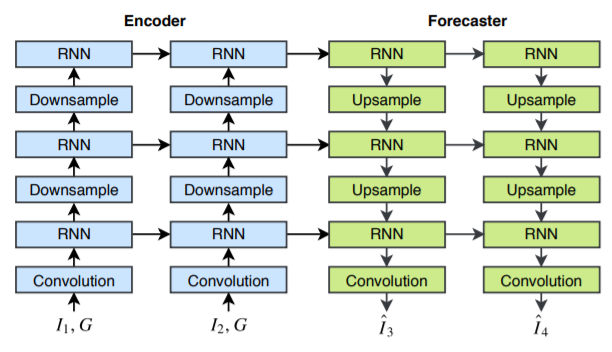
\includegraphics[width=\linewidth]{TrajGRU_EP}
\caption{Network description about encoder predictor in which $n=3$, $J=2$,$K=2$}
\end{figure}
Note that, in the predictor process, the flow is reversed because `The reason to reverse the order of the forecasting network is that the high-level states, which have captured the global spatialtemporal representation, could guide the update of the low-level states. Moreover, the low-level states could further influence the prediction.`

\subsection{Convolutional GRU}
The main formulas of the convGRU are given as follows:
\begin{equation}
\begin{split}
Z_t=\sigma(W_{xz}*X_t+W_{hz}*H_{t-1})\,\\
R_t=\sigma(W_{xr}*X_t+W_{hr}*H_{t-1})\,\\
H_t^{\prime}=LeakyRELU(0.2)(W_{xh}*X_t+R_t \circ (W_{hh}*H_{t-1}))\,\\
H_t=(1-Z_t)\circ H_t^{\prime}+Z_t \circ *H_{t-1}\\
\end{split}
\end{equation}
Among thiese equations, $\circ$ is the Hadamard product which also known as element-wise product, while $*$ stands for matrix convolution.

\subsection{Trajectory GRU}
The author takes the location into account by warp the specific location e.g. $i\,j \in N_{i,j}^h$ to new location i,j in the hidden state. This is achieved by the following formula.
\begin{equation}
H_{y,:,i,j}^{\prime}=f(W_{hh}concat(<H_{t-1,:,p,g} \vert (p,g) \in N_{i,j}^{h}>))=f(\sum_{l=1}^{\vert N_{i,j}^h \vert}W_{hh}^lH_{t-1,:,p_{l,:,i,j},g_{l,:,i,j}})
\end{equation}
$N_{i,j}^{h}$ is the ordered neighborhood set at location $(i,j)$ defined by the hyperparameters of the state-to-state convolution. L is the number of links connecting both location brefore warped and warped. The author plotted the links illustrated below. 

\begin{figure}[H]
\centering
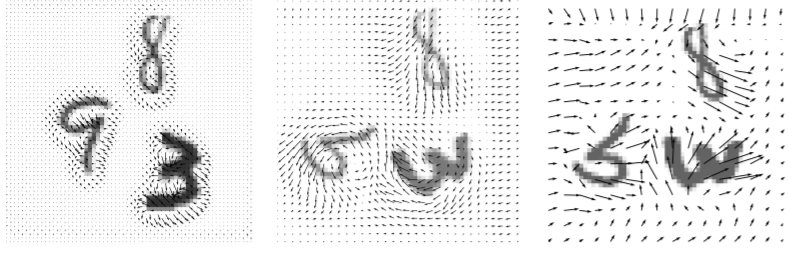
\includegraphics[width=\linewidth]{TrajGRU_res}
\caption{The plotted one of 13 links of arrow starting from each pixel to the pixel that is referenced by the link. From left to right are the first, second and third layer of the encoder. The link displayed has learned behavior of rotations}
\end{figure}

\section{Temporal Convolutional Neural Network for the Classification of Satellite Image Time Series}
This paper describes a major challenge to classify Satellite Image Time Series (SITS). Previously, the classification method has been done mainly rely on e.g. random forest (RF), SVM etc. which did not leverage the temporal behavior of the satellite data i.e. they can achieve the same performance with shuffled order.
\subsection{Key Points}
\begin{itemize}
\item a new framework TempCNNs for classification
\item exploring the architecture of TempCNNs.
\end{itemize}



\end{document}